\documentclass{beamer}

\mode<presentation> {

%\usetheme{default}
%\usetheme{AnnArbor}
%\usetheme{Antibes}
%\usetheme{Bergen}
%\usetheme{Berkeley}
%\usetheme{Berlin}
%\usetheme{Boadilla}
%\usetheme{CambridgeUS}
%\usetheme{Copenhagen}
%\usetheme{Darmstadt}
%\usetheme{Dresden}
%\usetheme{Frankfurt}
%\usetheme{Goettingen}
%\usetheme{Hannover}
%\usetheme{Ilmenau}
%\usetheme{JuanLesPins}
%\usetheme{Luebeck}
\usetheme{Madrid}
%\usetheme{Malmoe}
%\usetheme{Marburg}
%\usetheme{Montpellier}
%\usetheme{PaloAlto}
%\usetheme{Pittsburgh}
%\usetheme{Rochester}
%\usetheme{Singapore}
%\usetheme{Szeged}
%\usetheme{Warsaw}


%\usecolortheme{albatross}
%\usecolortheme{beaver}
%\usecolortheme{beetle}
%\usecolortheme{crane}
%\usecolortheme{dolphin}
%\usecolortheme{dove}
%\usecolortheme{fly}
%\usecolortheme{lily}
%\usecolortheme{orchid}
%\usecolortheme{rose}
%\usecolortheme{seagull}
%\usecolortheme{seahorse}
%\usecolortheme{whale}
%\usecolortheme{wolverine}

%\setbeamertemplate{footline} % To remove the footer line in all slides uncomment this line
%\setbeamertemplate{footline}[page number] % To replace the footer line in all slides with a simple slide count uncomment this line

%\setbeamertemplate{navigation symbols}{} % To remove the navigation symbols from the bottom of all slides uncomment this line
}

\usepackage{graphicx} % Allows including images
\usepackage{booktabs} % Allows the use of \toprule, \midrule and \bottomrule in tables
\usepackage{amsfonts}
\usepackage{mathrsfs}
\usepackage{amsmath,amssymb,graphicx, bm}

%----------------------------------------------------------------------------------------
%	TITLE PAGE
%----------------------------------------------------------------------------------------

\title["6.6"]{6.6: Regression with ARIMA errors} 

\author{Taylor} 
\institute[UVA] 
{
University of Virginia \\
\medskip
\textit{} 
}
\date{} 

\begin{document}
%----------------------------------------------------------------------------------------

\begin{frame}
\titlepage 
\end{frame}

%----------------------------------------------------------------------------------------

\begin{frame}
\frametitle{Motivation}

These are useful when you want to run a regression, but your errors are correlated.

\end{frame}

%----------------------------------------------------------------------------------------

\begin{frame}
\frametitle{Motivation}

Consider the model
\[
Y_t = x_t'\beta + W_t
\]
\[
\phi(B)W_t = \theta(B)Z_t, \hspace{5mm} \{Z_t\} \sim WN(0,\sigma^2)
\]
when $t=1,\ldots,n$
\newline

The linear regression you're used to assumes $W_t \sim WN(0,\sigma^2)$.
\end{frame}

%----------------------------------------------------------------------------------------

\begin{frame}
\frametitle{Ordinary Least Squares (the old way)}

Let's write this in matrix form: $\mathbf{Y} = \mathbf{X}\beta + \mathbf{W}$. When $\text{Var}(W) = \sigma^2 I$, we have
\[
(\mathbf{Y} - \mathbf{X}\beta )' (\mathbf{Y} - \mathbf{X}\beta ) = \sum_{t=1}^n (y_t - x_t'\beta)^2.
\]
Minimizing this gives you the {\bf ordinary least squares (OLS)} estimates of $\beta$.
\newline

\begin{enumerate}
\item $\hat{\beta} = (\mathbf{X}' \mathbf{X} )^{-1} \mathbf{X}'\mathbf{y}$
\item $E\hat{\beta} = \mathbf{\beta}$
\item $\text{Var}(\hat{\beta}) = \sigma^2 (\mathbf{X}' \mathbf{X} )^{-1} \mathbf{X}'\mathbf{X}(\mathbf{X}' \mathbf{X} )^{-1} = \sigma^2 (\mathbf{X}' \mathbf{X} )^{-1}$
\end{enumerate}



\end{frame}

%----------------------------------------------------------------------------------------

\begin{frame}
\frametitle{Generalized Least Squares (the new way)}

$\mathbf{Y} = \mathbf{X}\beta + \mathbf{W}$. When $\text{Var}(W) = \Gamma$, our loss function is
\[
(\mathbf{Y} - \mathbf{X}\beta )' \Gamma^{-1} (\mathbf{Y} - \mathbf{X}\beta ) .
\]
Minimizing this gives you the {\bf generalized least squares (GLS)} estimates of $\beta$.
\newline

\begin{enumerate}
\item $\hat{\beta} = (\mathbf{X}' \Gamma^{-1} \mathbf{X} )^{-1} \mathbf{X}'\Gamma^{-1}  \mathbf{y}$
\item $E\hat{\beta} = \mathbf{\beta}$
\item $\text{Var}(\hat{\beta}) = (\mathbf{X}' \Gamma^{-1} \mathbf{X} )^{-1} \mathbf{X}'\Gamma^{-1}\mathbf{X}(\mathbf{X}'\Gamma^{-1} \mathbf{X} )^{-1} = (\mathbf{X}'\Gamma^{-1} \mathbf{X} )^{-1}$
\end{enumerate}

Problem: $\Gamma$ is a function of $\phi$ and $\theta$, and so is unknown. The $\hat{\beta}$ depends on $\phi$ and $\theta$, which means it's usually unavailable.

\end{frame}
%----------------------------------------------------------------------------------------

\begin{frame}
\frametitle{Generalized Least Squares (the new way)}

If $\mathbf{Y} = \mathbf{X}\beta + \mathbf{W}$, $\text{Var}(W) = \Gamma$, then let $T'T = \sigma^2\Gamma^{-1}$. Then
\[
\tilde{\mathbf{Y}} = T'\mathbf{Y} = T'\mathbf{X}\beta + T'\mathbf{W} = \tilde{\mathbf{X}}\beta + \mathbf{e} 
\]
and we can use OLS (homework question). 
\newline

Cochran and Orcutt: ultiplying our data by $T'$ is similar to applying $\phi(B)$ to our data if $W_t$ is AR(p). We don't explore this further.

\end{frame}

%----------------------------------------------------------------------------------------

\begin{frame}
\frametitle{Generalized Least Squares (the new way) MLE}

Now pretend that we don't know the parameters $\phi$ and $\theta$. We look at a more complicated loss function.
\newline

We take negative twice the log of the following:
\[
L(\beta, \phi, \theta,\sigma^2) = (2 \pi)^{-n/2} (\det \Gamma)^{-1/2}\exp\left\{-\frac{1}{2} (\mathbf{Y} - \mathbf{X}\beta )' \Gamma^{-1} (\mathbf{Y} - \mathbf{X}\beta )  \right\}
\]

See how the previous procedure was a special case of this? 


\end{frame}

%----------------------------------------------------------------------------------------

\begin{frame}
\frametitle{Generalized Least Squares (the new way) MLE}

\begin{itemize}
\item Example 6.6.1 fits the model: $Y_t = \beta + W_t$ where $W_t$ is an MA(1) process.
\item Example 6.6.2 fits the model $Y_t = \beta_0 + \beta_1 t + W_t$ where $W_t$ is AR(2).
\item Example 6.6.3 fits the model $Y_t = \beta_0 + \beta_1 1(t \ge 99) + W_t$ where $W_t$ is MA(12)
\end{itemize}

\end{frame}

%----------------------------------------------------------------------------------------

\begin{frame}
\frametitle{Example 6.6.3}

If $Y_t = \beta_0 + \beta_1 1(t \ge 99) + W_t$ then 
\[
Y_t - Y_{t-12} = \beta_1 [1(t \ge 99) - 1(t-12 \ge 99)] + N_t 
\]
where $N_t = W_t - W_{t-12}$. So let's difference our data and fit the model:
\begin{block}{model}
\[
X_t = \beta g_t + N_t
\]
\end{block}
where $X_t = Y_t - Y_{t-12}$ and $g_t = 1(t \ge 99) - 1(t \ge 99+12) = 1( 99 \le t \le 110)$. 

\end{frame}

%----------------------------------------------------------------------------------------

\begin{frame}
\frametitle{Example 6.6.3}

$X_t = \beta g_t + N_t$ \\
Because we difference with lag 12, our dataset starts at $t=13$, meaning we only have $120-12=108$ datapoints. See 6.6.R.

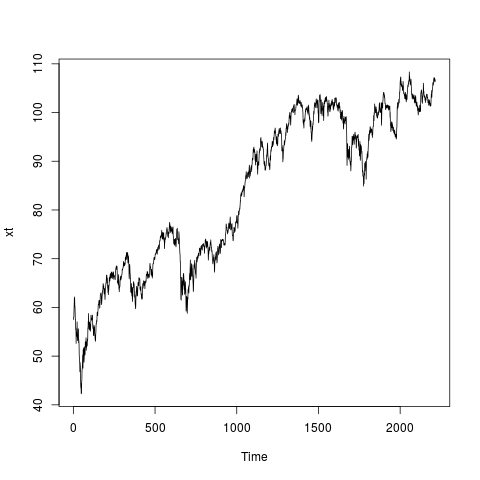
\includegraphics[width=43mm]{/home/taylor/UVa/all_teaching/4170_slides/6/6.6/pics/Rplot.png}
Red lines are the naive regression fitted values. The black lines are the better model's fitted values.

\end{frame}


\end{document} 